\begin{figure}[H]
	\centering
	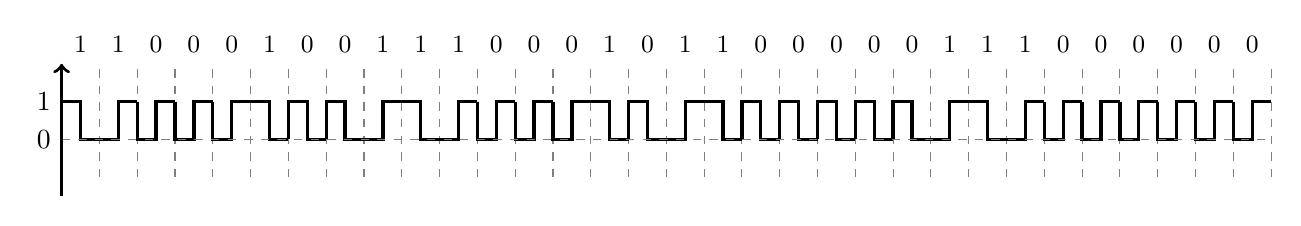
\begin{tikzpicture}[scale=0.48, very thick]
		\def\bits{1,1,0,0,0,1,0,0,1,1,1,0,0,0,1,0,1,1,0,0,0,0,0,1,1,1,0,0,0,0,0,0}

		\gdef\y{1}
		\foreach \b [count=\x from 0] in \bits {
			\draw[dashed, gray, thin] (\x+1,-1) -- (\x+1,2);
			\node at (\x+0.5, 2.5) {\small \b};
			\ifnum\b=0
				\ifnum\y=1
					\draw (\x,1) -- (\x,0) -- (\x+0.5,0) -- (\x+0.5,1) -- (\x+1,1);
					\xdef\y{1}
				\else
					\draw (\x,0) -- (\x,1) -- (\x+0.5,1) -- (\x+0.5,0) -- (\x+1,0);
					\xdef\y{0}
				\fi
			\else
				\ifnum\y=1
					\draw (\x,1) -- (\x+0.5,1) -- (\x+0.5,0) -- (\x+1,0);
					\xdef\y{0}
				\else
					\draw (\x,0) -- (\x+0.5,0) -- (\x+0.5,1) -- (\x+1,1);
					\xdef\y{1}
				\fi
			\fi
		}

		\draw[dashed, gray, thin] (0,0) -- (32,0);
		\draw[->] (0,-1.5) -- (0,2);

		\node[left] at (0,0) {0};
		\node[left] at (0,1) {1};
	\end{tikzpicture}
	\caption{Манчестерское дифференциальное кодирование исходного сообщения}
\end{figure}
